\documentclass{article}

\usepackage{amsmath, amsthm, amssymb, amsfonts}
\usepackage{thmtools}
\usepackage{graphicx}
\usepackage{setspace}
\usepackage{geometry}
\usepackage{float}
\usepackage{hyperref}
\usepackage[utf8]{inputenc}
\usepackage[english]{babel}
\usepackage{framed}
\usepackage[dvipsnames]{xcolor}
\usepackage[most]{tcolorbox}
\usepackage{minted}
\usepackage{amssymb}
\usepackage{indentfirst}
\usepackage{tabto}
\usepackage{soul}

\usepackage[export]{adjustbox} % Align images

\colorlet{LightGray}{White!90!Periwinkle}
\colorlet{LightOrange}{Orange!15}
\colorlet{LightGreen}{Green!15}

\newcommand{\HRule}[1]{\rule{\linewidth}{#1}}

\newtcbtheorem[auto counter,number within=section]{code}{Código}{
    colback=LightOrange!20,
    colframe=LightOrange,
    colbacktitle=LightOrange,
    fonttitle=\bfseries\color{black},
    boxed title style={size=small,colframe=LightOrange},
}{code}

\setstretch{1.2}
\geometry{
    textheight=22.5cm,
    textwidth=13.75cm,
    top=2.5cm,
    headheight=12pt,
    headsep=25pt,
    footskip=30pt
}

% ------------------------------------------------------------------------------

\begin{document}

% ------------------------------------------------------------------------------
% Cover Page and ToC
% ------------------------------------------------------------------------------
\begin{center}
    \begin{figure}
        
\includegraphics[scale = 0.3, left]{img/IST_A.eps} % IST logo
        \end{figure}
    \LARGE{ \normalsize \textsc{} \\
    [2.0cm] 
    \LARGE{ \Huge \textsc{Base de Dados}} \\
    [1cm]
    \LARGE{ \LARGE \textsc{LEIC-A IST-UL}} \\
    [1cm]
    \HRule{1.5pt} \\
    [0.4cm]
    \LARGE \textbf{\uppercase{Projeto BD - Parte 1}}
    \HRule{1.5pt}
    \\ [2.5cm]
    }
\end{center}

\vspace{0.5cm}
\makebox[\textwidth]{
    \textbf{\LARGE Grupo -- - BD---- - Daniela Falcão Machado}
}
\begin{center}
\begin{tabular}{ l c c c}
\textbf{Nome} & \textbf{Número} & \textbf{Contribuição} & \textbf{Esforço (Horas)} \\
 ------------ & --------- & 33.3\% & 8h \\
 ------------ & ---------  & 33.3\% & 8h \\
 ------------ & --------- & 33.3\% & 8h
\end{tabular}
\end{center}

\begin{center}
    \vspace{3.5cm}
    \date \large \bf  2023/2024 -- 2º Semester, P4
\end{center}


\setcounter{page}{0}
\thispagestyle{empty}

\newpage

% ------------------------------------------------------------------------------
% Table of Contents
% ------------------------------------------------------------------------------


\tableofcontents
\newpage

% ------------------------------------------------------------------------------
% Content
% ------------------------------------------------------------------------------



\section{Modelação Entidade-Associação}

\subsection{Modelo E-A}
\noindent
\makebox[\textwidth]{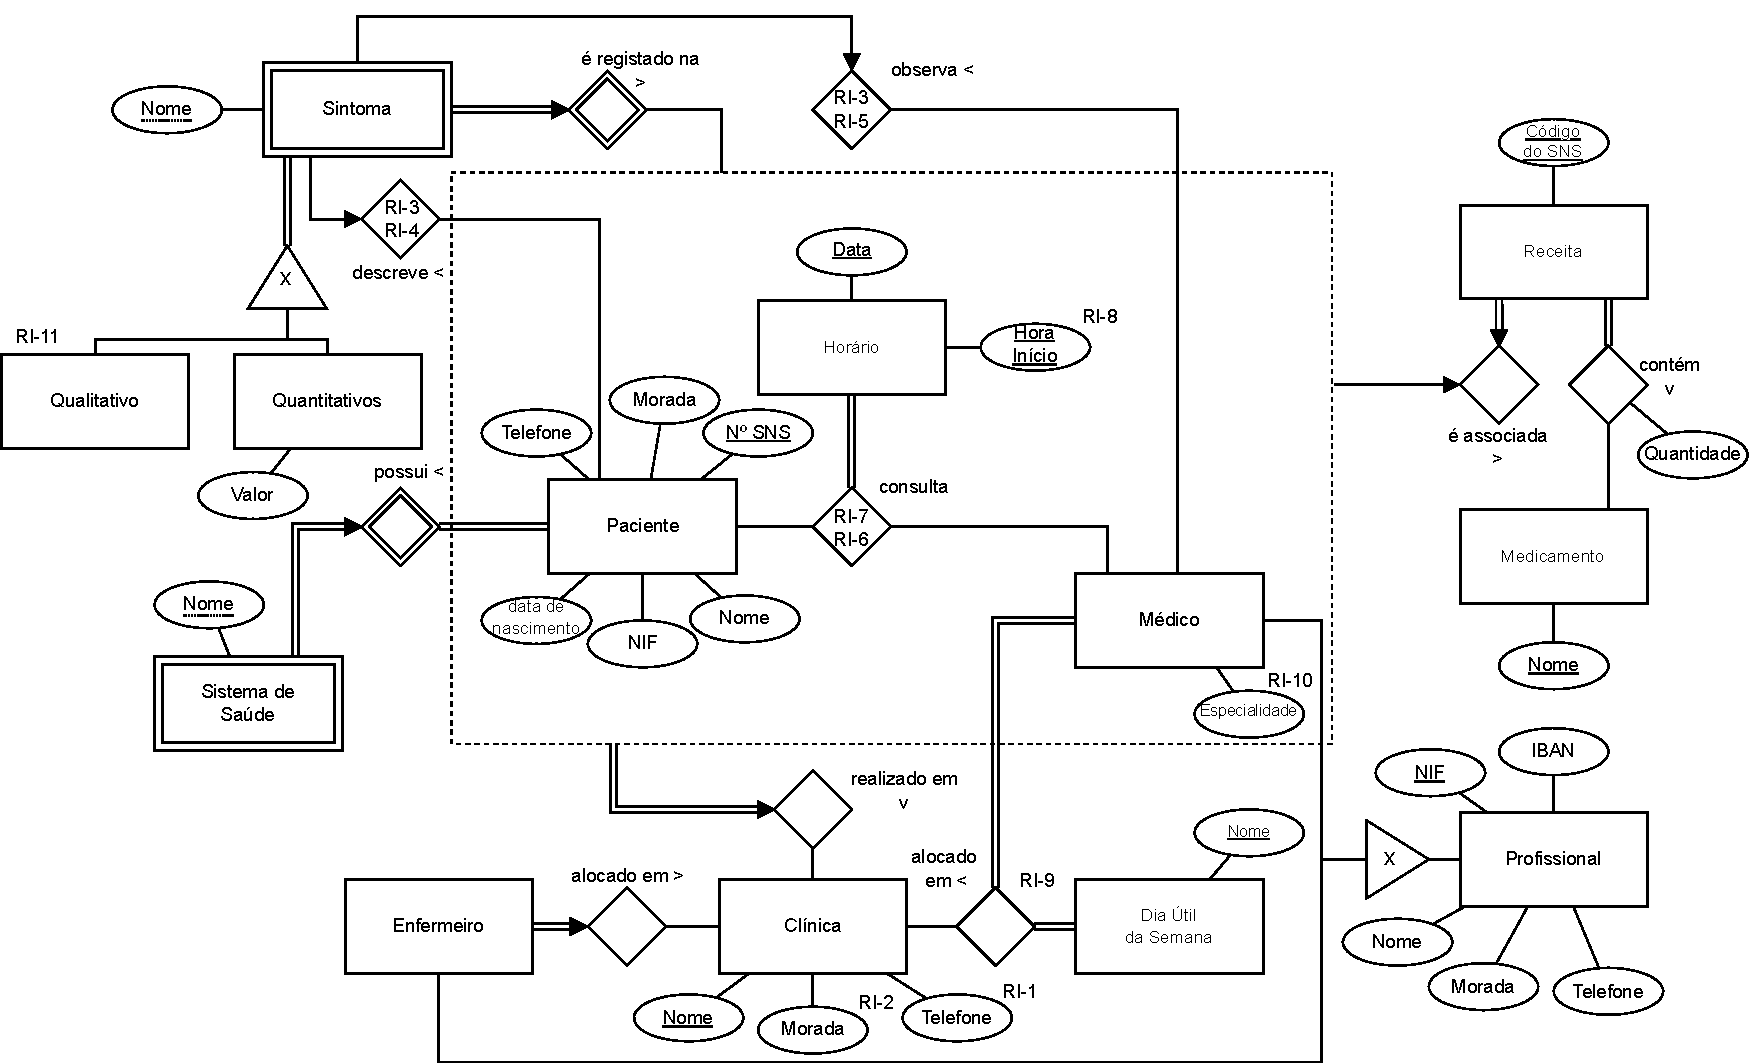
\includegraphics[scale = 0.6, center]{img/Diagrama.pdf}}

\subsection{Situações inconsistentes}
\begin{enumerate}
    \item Segundo o domínio as clínicas da empresa possuem um número de telefone único, mas no modelo E-A, como Telefone é um atributo não chave é possível ser repetido.
    \item Segundo o domínio as clínicas da empresa possuem uma morada única, mas no modelo E-A, como Morada é um atributo não chave é possível ser repetida.
    \item Segundo o domínio em cada consulta são registados sintomas descritos pelo paciente e/ou observados pelo médico, o que nos obriga a referir que um sintoma quando existe ou está associado a uma descrição por parte do paciente ou a uma observação por parte do médico, tendo que existir em pelo menos uma destas 2 associações.
    \item Segundo o domínio, um sintoma só pode ser descrito pelo paciente que está sujeito à consulta relevante, mas o modelo E-A permite a qualquer paciente descrever o sintoma de qualquer consulta, mesmo que doutro paciente.
    \item Segundo o domínio, um sintoma só pode ser observado pelo médico que efetua a consulta relevante, mas o modelo E-A permite a qualquer médico observar o sintoma de qualquer consulta., mesmo que doutro médico
    \item Num período de tempo, é contra o senso comum quer um paciente quer um médico ter mais que uma marcação, ou seja não pode haver pacientes ou médicos com consultas em horários sobrepostos, mas no modelo E-A não está contemplada essa restrição.
    \item É contra o senso comum o médico no dia útil da semana em que a consulta é realizada estar alocado a uma clínica que não seja na que a consulta é realizada, mas no modelo E-A não está contemplada essa restrição.
    \item Segundo o domínio a hora de início tem de ser entre as 8:00 e as 19:30, porque é um período de 30 minutos entre as 8:00 e as 20:00 mas no modelo E-A qualquer hora de início é permitida.
    \item Segundo o domínio, cada médico num determinado dia útil da semana está alocado a uma e apenas uma clínica, no entanto no modelo E-A é possível o médico estar em clínicas diferentes no mesmo dia, ou não estar em nenhuma nesse dia.
    \item Segundo o domínio, a especialidade dos médicos é escolhida de uma lista de especialidades reconhecidas, mas no modelo E-A não existe essa restrição. 
    \item Segundo o domínio, os medicamentos são escolhidos da lista oficial do Infarmed, contudo no modelo E-A não existe essa restrição.
\end{enumerate}

\subsection{Restrições de Integridade}
Seguem das situações inconsistentes anteriores, as seguintes Restrições de Integridade correspondentes: 
\begin{itemize}
  \item RI-1 - O Telefone é único para cada entidade Clínica
  \item RI-2 - A Morada é única para cada entidade Clínica
  \item RI-3 - Sintoma tem de participar em pelo menos numa destas associações
  \item RI-4 - Sintoma só pode ser descrito por Paciente da consulta em que ele é registado
  \item RI-5 - Sintoma só pode ser observado por Médico da consulta em que ele é registado
  \item RI-6 - O mesmo Médico, ou Paciente não pode estar associado a Horários com uma Hora de Início menos de 30 minutos de diferença
  \item RI-7 - Médico no Dia Útil da Semana correspondente à Data tem de estar alocado à clínica em que o serviço de saúde é realizado
  \item RI-8 - Hora de início está entre as 8:00 e 19:30
  \item RI-9 - Cada par Médico Dia Útil da Semana é único e existe na relação
  \item RI-10 - Especialidade é uma das especialidades reconhecidas pela ordem dos médicos
  \item RI-11 - Nome do sintoma está presente na lista do vocabulário controlado SNOMED CT
\end{itemize}

\section{Conversão E-A–Relacional}

A(\underline{a1}, a2, a3)

B(\underline{a1}, b1) 

\quad a1: FK(A)

C(\underline{a1})

\quad a1: FK(A)

E(\underline{e1},\underline{e2})

rCE(\underline{a1},e1,e2,rce1)

\quad a1: FK(C)

\quad e1,e2: FK(E) NOT NULL

F(\underline{f1},\underline{f2},f3)

G(\underline{g1})

H(\underline{h1}, h2) 


rAFG(\underline{a1}, \underline{f1}, \underline{f2}, g1, h1)

\quad a1: FK(A)

\quad f1, f2: FK(F)

\quad g1: FK(G) NOT NULL

\quad h1: FK(H) NOT NULL


D(\underline{d1}, \underline{a1}, \underline{f1}, \underline{f2})

\quad a1, f1,f2: FK(rAFG)

\subsection{Restrições não passíveis de conversão}
\begin{enumerate}
\item Para representar a especialização da entidade A do diagrama E-A foi escolhido mapear todas as entidades (A, B, C) como relações, mas neste caso é possível ocorrer uma chave de A em B e C em simultâneo, ou não ocorrer nem em B nem em C, ou seja é uma especialização livre em vez de disjunta total.
\item Apesar de no diagrama E-A a Entidade F ter uma participação obrigatória na associação rAFG, é possível uma chave de F não estar na relação rAFG.
\item E apesar de no diagrama E-A a Entidade H ter uma participação obrigatória na associação rHrAFG, é possível no modelo relacional uma chave de H não estar na relação rAFG.
\end{enumerate}

\subsection{Restrições de Integridade}
Seguem das situações inconsistentes anteriores, as seguintes Restrições de Integridade correspondentes: 
\begin{itemize}
    \item RI-1: Cada chave de A tem de ocorrer em B ou em C mas não em ambos
    \item RI-2: Todas as instâncias de F têm de existir na relação rAFG
    \item RI-3: Todas as instâncias de H têm de existir na relação rAFG
\end{itemize}

\section{Álgebra Relacional \& SQL}

\subsection{Expressão de álgebra relacional}
Expressão que corresponde à interrogação "quais os pacientes que
consultaram médicos de todas as especialidades?":

\ul{$\Pi_{\text{SSN,especialidade}}(\text{consulta}\bowtie_{\text{consulta.NIF=medico.NIF}}\text{medico})\div\Pi_{\text{especialidade}}(\text{medico})$}

\subsection{Interrogação em linguagem natural}

\noindent $r\xleftarrow{}_{\text{especialidade}}G_{\text{count()}\xrightarrow{}\text{consultas}}(\text{consulta}\bowtie_{\text{consulta.NIF=medico.NIF}}\text{medico})$ \\
$\Pi_{\text{especialidade}}(\text{medico})-\Pi_{\text{r1.especialidade}}(\sigma_{\text{r1.consultas}<\text{r2.consultas}}(\rho_{\text{r1}}\text{r}\times\rho_{\text{r2}}\text{r}))$ \\

r é o número de consultas feitas em cada especialidade e a segunda expressão é todas as especialidades exceto as especialidades em que existe outra especialidade com um número maior de consultas, ou seja:

\ul{“Sobre qual especialidade é realizada o maior número de consultas?”
}


\subsection{Interrogação em linguagem natural}
\ul{“Quais são os SSN’s e nomes dos pacientes que têm mais que uma consulta na mesma data?”}


\subsection{Expressão SQL apresentada pelo ChatGPT}
O resultado não representa de todo a resposta pretendida, logo não está semanticamente correta face à interrogação "Qual  médico tem pacientes mais fiéis?".

\begin{itemize}
    \item Primeiro, após a cláusula de \texttt{FROM} e dos \texttt{INNER JOIN}s é selecionado com um \texttt{WHERE} apenas a primeira consulta (devido ao \texttt{MIN(periodo)}) que um médico teve com um determinado paciente.
    \item Depois sobre esta tabela é executado um \texttt{GROUPBY} pelo nome do médico, o que não é de todo desejado, pois o que identifica o médico é o seu NIF e o seu nome, isto pode fazer com que médicos com o mesmo nome sejam considerados o mesmo.
    \item A seguir o \texttt{SELECT} cria as colunas consultas\_medico e total\_pacientes e devido à cláusula \texttt{WHERE} mencionada anteriormente, consultas\_medico não representa o número de consultas que cada médico efetuou, mas sim o número de primeiras consultas com um paciente, que é igual ao número de pacientes, ou seja  consultas\_medico = total\_pacientes, logo a proporcao\_fidelidade é constante, ou seja 1.0.
    \item De qualquer forma não foi comparado o número de idas do paciente a médicos da mesma especialidade.
    \item Finalmente, o resultado esperado era um médico, e não uma lista de médicos, deveria ser selecionado o NIF do médico com maior proporcao\_fidelidade.
\end{itemize}

\newpage

% ----------------------------------------------------------------------
% Cover
% ----------------------------------------------------------------------

\end{document}
